
\section{Kältetechnik}
\label{sec:Kaeltetechnik}

Die Kältetechnik wird in verschiedensten Einsatzgebieten eingesetzt, um Kälte zu erzeugen bzw. einem definierten Raum Energie in Form von Wärme zu entziehen. 

Das Konservieren von Lebensmittel ist  der ursprüngliche Hauptzwecke der Kältetechnik und ist auch heute noch aktuell. Bereits 3000 Jahre v. Chr. nutzten die Ägypter und Mesopotamier Natureis, um ihre Nahrungsmittel länger haltbar zu machen.\citep{Danfoss2006}

Im Jahre 1834 meldete der US-Amerikaner Jacob Perkins sein Patent zum Thema Kältetechnik in England an. Das Patent beschreibt eine Kaltdampfmaschine in einem geschlossenen Kreislauf mit dem feuergefährlichen Äthyläther als Kältemittel.\citep{Siemens2007}

Carl von Linde baute nach konstruktiven Verbesserungen der Kaltdampfmaschine und Verwendung von Ammoniak als Kältemittel im Jahre 1876 die erste praxistaugliche Kälteanlage. Die ersten Anlagen wurden durch die Maschinenfabrik Augsburg-Nürnberg gebaut und an Brauereien sowie später auch an die Schifffahrt vertrieben.

Mit steigender Bedeutung von Elektrizität als Energieträger nach dem 1.Weltkrieg nahm auch die Entwicklung und der Bedarf an Kälteanlagen zu. Im Jahre 1920 startet die Firma \textit{General Electric} mit der Serienherstellung von Haushaltkühlschränken mit Hermetik-Verdichtern.

Das vielseitige Gebiet der Kältetechnik umfasst alle Technologien, die zur Bereitstellung von Kälteenergie dienen. Sie unterscheiden sich in der benötigten zuzuführenden Energien, Einsatzbereich und eingesetzten Kältemitteln.  Zu den wichtigsten und heute meist verwendeten Technologien gehören folgende Technologien

\begin{itemize}

\item Kompressions-Kälteprozess: \textit{Prozess wird angetrieben durch Zufuhr mechanischer Energie}
\item Sorptions-Kälteprozess: \textit{Prozess wird angetrieben durch Zufuhr von Wärmeenergie}
\item Linde-Verfahren.

\end{itemize}

Weitere nicht so weitverbreitete Technologien der Kältetechnik, jedoch technisch interessante Verfahren  sind zB. das  \textit{Wirbelrohr},  \textit{Magnetische Kühlung} oder das Kühlen mittels einem Peltier-Element. Diese Verfahren werden meist nur unter hohem Energieverbrauch in Sonderfällen angewandt. \citep{Grote2014}

Da sich diese Masterarbeit mit dem Aufbau eines Prüfstandes zur Untersuchung von Abtaumethoden einer Kompressionskälteanlage beschäftigt, wird in den folgenden Kapitel ausschließlich auf diese Technologie eingegangen. Für weitere Informationen bezüglich der anderen Technologien sei an dieser Stelle auf die Literatur \citep{Baehr2013}, \citep{Grote2014} und \citep{Grote2014} verwiesen.



\subsection{Komponenten eines Kaltdampfprozesses}
\label{subsec:Komponenten eines Kaltdampfprozesses}

Die Komponenten für einen einfachen Kaltdampfprozess  besteht aus vier Komponenten:

\begin{itemize}
\item der Kompressor
\item der Verflüssiger 
\item das Drosselvenil Expansionsventil
\item der Verdampfer. 
\end{itemize}

In Abbildung \ref{fig:einfacher Kältekreislauf} sind die vier Komponenten mit ihren Zustandspunkten dargestellt.

\begin{figure}[htb]
\centering		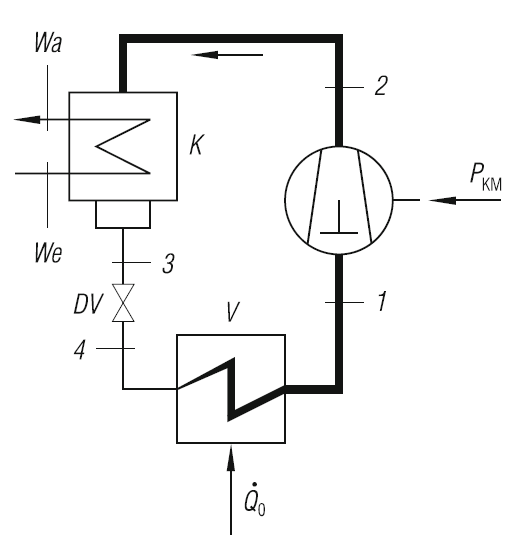
\includegraphics[width=0.50\textwidth]{Pictures/Kaltekreislauf_beahr.png}
\caption{Einfacher Kältekreislauf \citep{Baehr2013}}
\label{fig:einfacher Kältekreislauf}
\end{figure}

\subsubsection*{Der Kompressor}
Der Kompressor bildet das Herzstück der Kälteanlage. Er verdichtet das gasförmige Kältemittel von niedrigem Druck auf ein höheres Druckniveau. Um diese Arbeit zu verrichten, wird der Verdichter mit elektrischer Energie versorgt. Der Kompressor gibt es in verschiedenen Bauvarianten. Die zwei wichtigsten Bauvarianten sind der \textit{Hubkolbenverdichter} und der \textit{Rotationskolbenverdichter}. Die Baugruppen der Verdichter werden in offene, halbhermetische und vollhermetische Verdichter unterschieden. Schrauben-,Scroll- sowie Turboverdichter sind Bauarten der \textit{Rotationskolbenverdichter}. 



Ein wichtiges Kriterium bei Verdichtern ist das Druckverhältnis von Ansaugdruck, vor der Kompression, und dem Ausgangsdruck. Das Druckverhältnis $\pi$ ist definiert als:



\begin{equation}
\pi := \frac{p_{aus}}{p_{ein}}.
\label{Druckverhältnis}
\end{equation}

\subsubsection*{Der Verflüssiger}

Dem Kältemittel wird im Verflüssiger auf einem hohen Druckniveau Wärme entzogen. Der Verflüssiger kühlt das überhitzte, gasförmige Kältemittel ab. Beim Austritt aus dem Verflüssiger ist das Kältemittel meist vollständig kondensiert. 
Um einen Wärmeentzug zu bewerkstelligen gibt es drei Bautypen:

\begin{itemize}
\item Wassergekühlte Verflüssiger
\item Luftgekühlte Verflüssiger
\item Verdunstungsverflüsssiger
\end{itemize}

Wassergekühlte Verflüssiger können, aufgrund der besseren Wäärmeübertragung verglichen zu Luft, sehr kompakt gebaut werden. Eine typische Bauform ist das \textit{Bündelrohrverflüssiger}.
In der Praxis werden am häufigsten luftgekühlte Verflüssiger eingesetzt. Um die gleiche Kühlleistung wie ein wassergekühlter Verflüssiger zu erreichen, werden Lamellen und Ventilatoren eingesetzt. Die Lamellen vergrößern die Fläche für die Wärmeübertragung mit der Luft. Ventilatoren ermöglichen durch einen höheren Luftdurchsatz und der daraus resultierendem höhere Wärmeübertragung eine größere Kühlleistung und eine kompaktere Bauform der Wärmeübertragers. Diese Variante hat den Vorteil, dass die einen wartungsfreien Betrieb  sowie eine einfache Reinigung ermöglicht.


\subsubsection*{Das Expansionsventil}

Das Expansionsventil versorgt den Verdampfer mit dem nötigen Kältemittel-Massenstrom. Die Zuführung des Kältemittels erfolgt über eine Druckdifferenz. Durch eine lokale Verengung des Strömungquerschnitts, verringet sich der Druck des durchfließenden Kältemittels. Das Kältemittel vergrößert sein Volumen und es kommt zur Expansion. Die Druckreduzierung erfolgt ohne zusätzliche Arbeit. Im idealen Fall wird bei diesem Prozess auch keine Wärme abgefuhrt; der Prozess ist \textit{isenthalb}. 
Das Expansionsventil trennt zusammen mit dem Kompressor die zwei Druckseiten des Kältekreislaufes. Es gibt Expansionsventile sowohl als regelbare und nicht regelbare Ausführungen. Bei kleineren Anlagen erfolgt die Expansion ungeregelt zum Beispiel durch Kapillarrohre. Geregelte Expansionsventile werden in mittleren und großen Kälteanlagen eingesetzt. Die Regelung erfolgt durch die Querschnittsänderung und dem damit einhergehendem Druckabfall.  

\subsubsection*{Der Verdampfer}

In dem Verdampfer wird das Kältemittel eingespritzt. Das Kältemittel verdampft und entzieht seiner Umgebung dabei Wärme. Aufgrund der vielfältigen Anforderungen an Verdampfer, gibt es eine Vielzahl an Bauarten für Verdampfer. Mögliche Bauarten sind 

\begin{itemize}
\item Glattrohrverdampfer
\item Beripptes Verdampferregister
\item Rippenrohrverdampfer
\end{itemize}

Um eine möglichst große Kälteleistung zu ermöglichen, werden wie beim Verflüssiger auch, Ventilatoren eingesetzt. Die Ventilatoren erzwingen einen Luftstrom durch den Verdampfer und erhöhen damit die Wärmeübertragung zwischen der Luft und den Verdampferrohren. 

%\newpage
\subsection{Abtaumethoden}
\label{subsec: Abtaumethoden}

Um einen vereisten Luftkühler abzutauen, gibt es mehrere Methoden. Die Methoden unterscheiden sich in der Installation, Schnelligkeit, Effizienz und Effektivität. Je nach Einsatzbereich und Anlage wird entschieden welche Abtaumethode installiert und eingesetzt wird. Mehrkosten für die Installation sowie weitere Betriebskosten sind bei der Entscheidung stets ein nicht zu vernachlässigender Punkt.
Die in der Praxis am weit verbreitesten Methoden sind  die \textit{Heißgas-Abtauung}, \textit{Prozessumkehrung}, \textit{elektrische Abtauung} und \textit{Umluft-Abtauung}.

Die Tabelle \ref{tab:Vor- und Nachteile} gibt einen Überblick über die Vor- und Nachteile der jeweiligen Abtaumethode. 

\subsubsection*{Heißgas-Abtauung}

Die Heißgasabtaung wird durchgeführt indem das Heißgas aus dem Kompressor anstatt in den Verflüssiger direkt in den vereisten Verdampfer leitet. Für diese Methode wird eine Bypass-Leitung von dem Austritt vom Verdichter bis zum Eingang des Expansionsventil gelegt. Mittels zwei Drei-Wegeventilen kann diese Leitung geöffnet bzw. geschlossen werden. In der Abtauphase ist der Verflüssiger vom Kreislauf ausgeschlossen, damit kein flüssiges Kältemittel in den Verdampfer fließt. \citep{Baehr2013}
Der Prozess läuft in 3 Schritten ab:

\begin{itemize}
\item[1$\longrightarrow$ 2] Kältemittel-Verdichtung durch den Kompressor unter Aufnahme elektrischer Energie

\item[2 $\longrightarrow$ 3] Isenthalpe Entspannung durch das Expansionsventil

\item[3 $\longrightarrow$ 1] Wärmeabgabe an Rohre, Lamellen und das Eis. 
\end{itemize}


In Abbildung \ref{fig:Heissgas-Abtauung} ist der rechtsläufige Kreisprozess in einem ln p, h- Diagramm für das Kältemittel R290 abgebildet. 


\begin{figure}[htb]
\centering
\subfigure[Fließbild. Links: Kühlbetrieb, Rechts: Abtaubetrieb]
{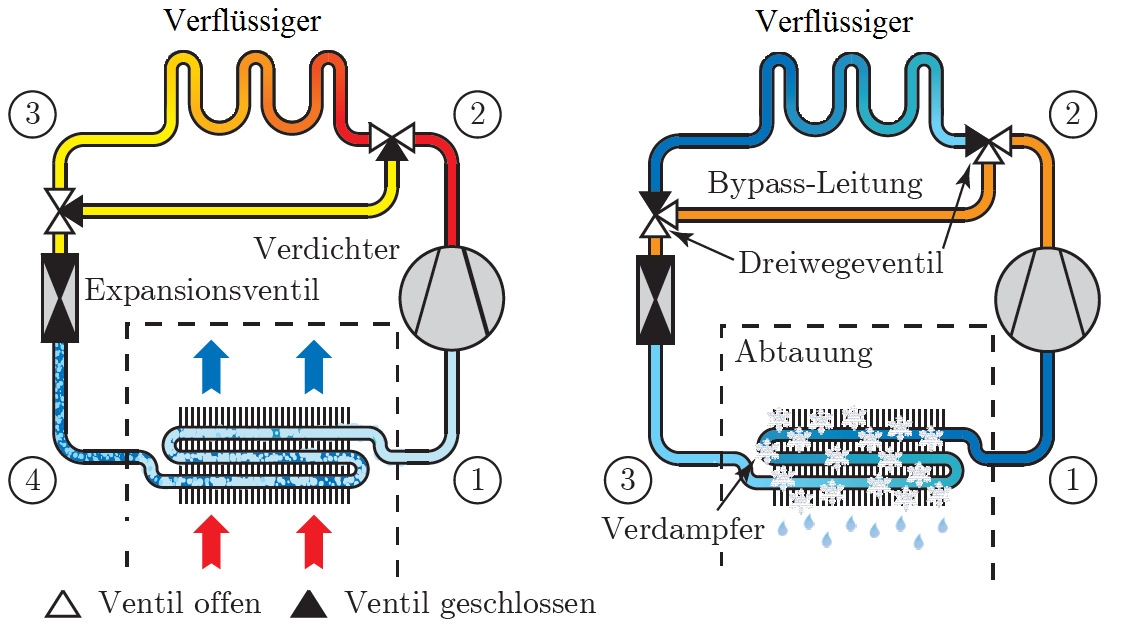
\includegraphics[width=0.640\textwidth]{Pictures/HeissgasKosowski.png}}
\subfigure[Zustandspunkte im ln p,h Diagramm]{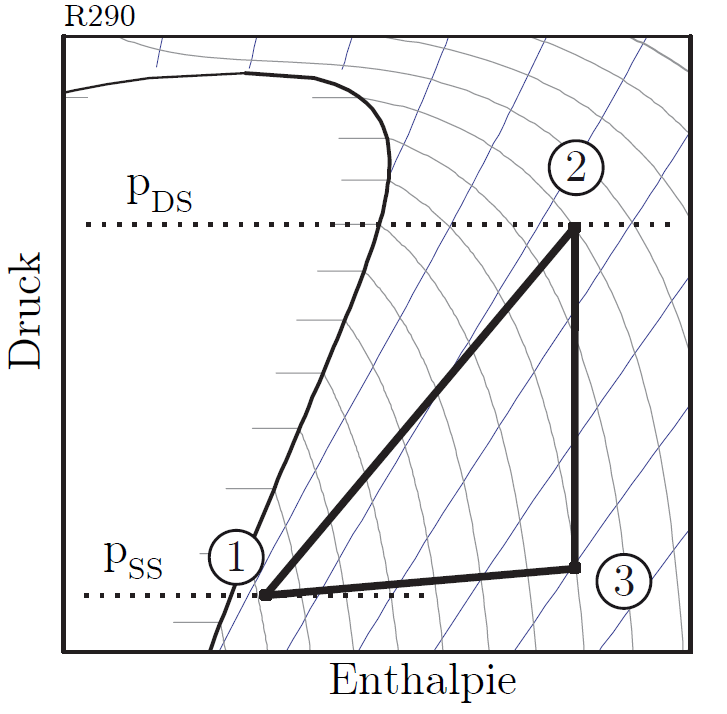
\includegraphics[width=0.35\textwidth]{Pictures/HeissgasEnthalpieDiagrammKosowski.png}}
\caption{Heißgas-Abtauung \citep{Kosowski2009}}
\label{fig:Heissgas-Abtauung}
\end{figure}



\subsubsection*{Prozessumkehrung}

Bei der Abtauung durch Prozessumkehrung wird die Funktion der Wärmeübertrager vertauscht. Während des Abtauprozesses fungiert der Verdampfer als Verflüssiger und der Verflüssiger hat die Aufgabe des Verdampfers inne. Die Prozessumkehrung wird in der Regel durch ein Vierwegeventil gewährleistet. Das Vierwegeventil wird bei der Abtauung geschaltet und leitet das Kältemittel nach dem Kompressor erst in den vereisten Verdampfer. Das überhitzte Kältemittel durchströmt den Verdampfer auf hohem Druckniveau und gibt Wärme an die Rohre und Lamellen des Luftkühlers sowie an das Eis ab.

Die Versuchsalage, die in dieser Arbeit optimiert worden ist, ist mit dieser Technologie ausgestattet. Der Umkehrprozess wird näher im Kapitel \ref{cha: Versuchsaufbau} erläutert. 


\begin{figure}[htb]
\centering		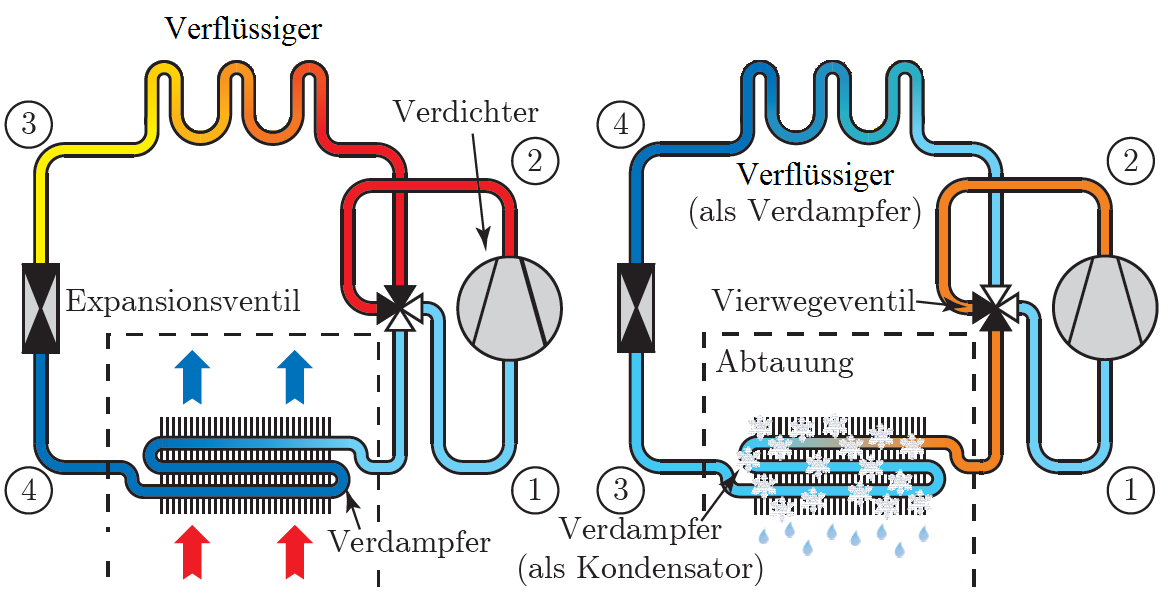
\includegraphics[width=0.7\textwidth]{Pictures/Prozessumkehrung_Kosowski.png}
\caption{Links: Kühlbetrieb. Rechts:Heißgas-Abtauung \citep{Kosowski2009}}
\label{fig:Prozessumkehrung}
\end{figure}

\subsubsection*{Elektrische Abtauung}

Eine weitere Möglichkeit der Abtauung ist die elektrische Abtauung. Bei dieser Methode sind Widerstandsheizungselemente in den Wärmeübertrager des Verdampfers installiert. Die Widerstandsheizung wandelt elektrische Energie in thermische Energie um, und überträgt diese weiter an den Wärmeübertrager und das Eis. 

Das Prinzip der Widerstandsheizung beruht auf einen niedrig ohmigen Widerstand, der von Strom durchflossen wird und sich dabei erhitzt. Die Widerstandsheizung, auch Heizpatronen genannt, können in Reihe oder auch parallel geschaltet werden. Bei der Erhitzung  Die abfallende elektrische Spannung über einen Heizswiderstand errechnet sich nach dem Ohmischen-Gesetz zu :

\begin{equation}
U = R I
\label{eq: Ohmisches Gesetz}
\end{equation}

Hierbei ist $R$ der spezifsche Widerstand des eingesetzen Material, meistens Metalle,  und $I$ die angelegte Stromstärke. Ein Heizwiderstand hat einen Wirkungsgrad von 100 $\%$ und wandelt somit die komplette elektrische Leistung in thermische um:

\begin{equation}
\dot{Q}_{th}= P_{el }= U I = \frac{U^2}{R} =  R I^2 
\label{eq:Leistung Heizwiderstand}
\end{equation}

Die thermische Leistung ist folglich proportional zu der angelegten Spannung $U$. Die Widerstände sind über die Spannung $U$ regelbar. Der Wärmeübergang von den Heizpatronen auf den Wärmeübertrager ist entscheidend für ein effizientes Abtausystem. Je formschlüssiger die Heizpatronen in den Verdampfer installiert sind, desto besser der Wärmeübergang und effizienter die Abtauuung.  
Die Versuchsanlage dieser Arbeit ist auch mit dieser Abtautechnologie ausgestattet. 

\subsubsection*{Umluft-Abtauung}

Die Umluft-Abtauung ist eine weitere in der Praxis häufig verwendete Abtaumethode. Hierbei wird der Verdampfer durch die vorbeiströmende Umluft abgetaut. Um dies zu ermöglichen muss zum einen der Ventilator in der Abtauphase laufen und zum anderen die Umgebungstemperatur größer als 0 $°$C sein. Ein Vorteil dieses Verfahrens ist, dass die Wärmeübertragung luftseitig geschieht und dadurch die zuzuführende Wärme nicht zusätzlich das Material des Verdampfers erhitzen muss. 

Diese Abtaumethode wird in der Arbeit nicht näher untersucht. Deswegen wird an dieser Stelle auf die  Literaturquellen \citep{Breidenbach2014} und \citep{Ehrbar2002} verwiesen. 

%\subsubsection{Gegenüberstellung der Abtaumethoden}
%\label{subsubsec:Gegenüberstellung }



%\begin{landscape}

\begin{table}[htb]
\centering
\caption{Vor- und Nachteile der verschiedenen Abtaumethoden   	\citep{Breidenbach2014}, \citep{Refrigeration2000}, \citep{Yin2012}, \citep{Huang20091697}
} \vspace{6pt}

\label{fig:PCM_Slurry1}
%\begin{tabular}{p{3.9cm}p{8cm}p{8cm}lll} 
\begin{tabular}{p{3.8cm}p{5.6cm}p{5.6cm}lll}
\hline
\textbf{Abtaumethode} &\textbf{Vorteile} & \textbf{Nachteile}\\
\hline
\hline

\textbf{Heißgas-Abtauung} 
&
$\bullet$ Guter Wärmeübergang zwischen Heißgas,Rohre und Eis
\newline								  			
$\bullet$ Unkomplizierte Wartung
\newline			  
$\bullet$ Kurze Abtaudauer		
\newline			
$\bullet$ Schnelles Wiederanfahren möglich	

&$\bullet$ Höherer Planungs- und Installationsaufwand  
\newline
$\bullet$ Zusätzliche Kühlung des Kompressors in Abtauphase ist erforderlich 
\newline 
$\bullet$ Höhere Druckverluste durch zusätzliche Komponenten 
\newline
$\bullet$ kritische Kältemittel-Menge bestimmt durch Abtauleistung \\  
   
\hline
\textbf{Prozessumkehrung}
&$\bullet$ Guter Wärmeübergang zwischen Heißgas,Rohre und Eis  													
\newline								
$\bullet$ Unkomplizierte Wartung
\newline	
$\bullet$ Kurze Abtaudauer		
\newline			 
$\bullet$ geeignet für Verbund-Systeme		
&$\bullet$ Abtropfwanne ist nicht beheizt   
\newline
$\bullet$ Höherer Planungs- und Installationsaufwand
\newline
$\bullet$ Nicht nachrüstbar
\newline
$\bullet$ Höhere Druckverluste durch zusätzliche Komponenten								
\newline
$\bullet$ Kritische Kältemittel-Menge bestimmt durch Abtauleistung\\


\hline
\textbf{Elektrische Abtauung }
&$\bullet$ Einfache Komponenten und Installation 
\newline 
$\bullet$ \textit{Stand-Alone}-System ist nachrüstbar		
\newline
$\bullet$ Hohe Regelgenauigkeit	
\newline
$\bullet$ Abtropfwanne ist beheizbar 					
&
$\bullet$ Schlechter Wärmeübergang 
\newline					
$\bullet$ Verursacht Kältemittelbewegung in den Sammler
\newline 
$\bullet$ Brandgefahr im Falle von Kabelbruch  
\newline
$\bullet$ Zeitliche Verzögerung beim Abtauprozess 
\newline
$\bullet$ Hohe thermische Belastung der Komponenten    
\\

 
\hline
\textbf{Umluft-Abtauung }
&
$\bullet$	Keine zusätzlichen Komponenten nötig			 
\newline
$\bullet$	Günstig										
\newline
$\bullet$	Keine zusätzlicher Wärmeeintrag ins System	  
\newline
$\bullet$	Keine Abtauung der Abtauwanne möglich	
&
$\bullet$ Bei überdimensionierten Kompressoren sehr hohe Abtaudauer möglich
\newline
$\bullet$ Funktioniert nur mit Umgebungstemperaturen über $ 2\,^{\circ}\mathrm{C} $
\\
\hline

\end{tabular}
\label{tab:Vor- und Nachteile}
\end{table}
%\end{landscape}
